\chapter{Results and discussion}
\section{Environments}

First environment used for evaluation is the \emph{Slimevolley} environment. The Slimevolley environment \cite{slimevolleygym} is based on a game called "Slime Volleyball" created by an unknown author. The agent's task in this environment is to get the ball to hit ground on the opponent's side to make the oponent lose a life. The opponent is controlled by a small, 120-parameter, pre-trained neural network. \cite{ha2015slimevolley}

Each agent has 5 lives in the beginning and the episode ends after 3000 steps or when either agent loses or their lives, whichever comes first. The agent receives a reward of $+1$ point when the opponent loses a life and $-1$ if it loses the life. In addition to this, for each survived timestep, the agent receives $+0.01$  reward. State is represented as a vector with 12 entries, $x$ and $y$ positions and respective velocities of the agent, opponent and the ball. Actions are represented as a vector with 3 entries, one for each action that the agent can do, jump, go forward or go backward. The agent will perform an action when the appropriate value is higher than 0.

\begin{figure}[h]
    \caption{Screenshot of Slimevolley environment}
    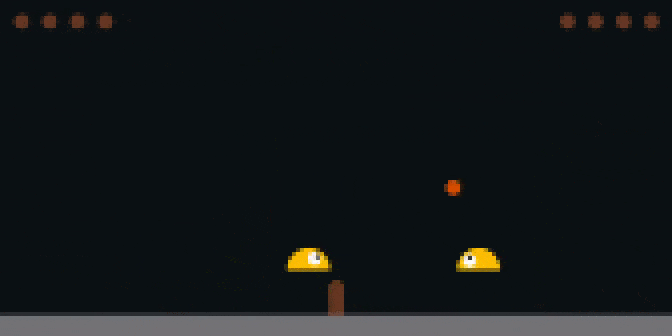
\includegraphics[width=0.8\textwidth]{img/slimevolley.png}
\end{figure}

Second environment is a \emph{Cartpole-swingup} environment. It is inspired by classic reinforcement learning benchmark task, pole-balancing. In this task one end of a pole is attached to a card which moves left and right and the goal is to keep the pole upright. In the original the episode ends when the pole is tilted too much off its neutral position. However in this version the pole is able to rotate $360^\circ$ and the episode ends only if the cart goes out of bounds or 1000 timesteps goes past.

The physics of the pole is controlled by equations specified for "Pendullum Swing-up" in PILCO software package \cite{pilco2013}. Reward is given based on how far is the cart from centre (closer is better) and what is the angle of the pole (more upright is better). State is represented with a 4-entry vector containing the position of the cart, its velocity, sine and cosine of the pole's angle and its angular velocity while action is a number from -1 to 1 which represents force which is applied, in either direction, to the cart.

\begin{figure}[h]
    \caption{Screenshot of Cartpole-swingup environment}
    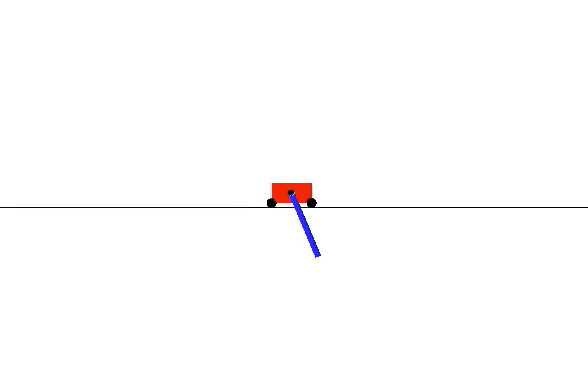
\includegraphics[width=0.8\textwidth]{img/cartpole.png}
\end{figure}

